
\begin{frame}{Approche générale de la méthode en 2D}
    \centering
    \textbf{Paramétrisation globale}
    
    %\vspace{1em}
    
    \begin{figure}
        \includegraphics[width=1.\linewidth]{img/new_images/gp_arrow_ex.png}
    \end{figure}

    \begin{itemize}
        \item Paramétrisation $f$ d'un domaine 2D vers une grille régulière.
        \item $f^{-1}$ permet de déposer la grille sur le domaine initial.
    \end{itemize}
\end{frame}

\begin{frame}{Méthode Quadcover pour calculer un maillage quadrilatère}
    \begin{columns}[c] % align columns
        
        \begin{column}{.7\textwidth}
            \textbf{Méthode utilisant un champ de repère}
            \vspace{1em}
            \begin{enumerate}
                \item Calcul champ de repère
                \begin{itemize}
                    \item Oriente les quadrilatères
                    \item Positionne les singularités
                \end{itemize}
                \vspace{.5em}
                \item Algorithme Quadcover
                \begin{itemize}
                    \item Calcule une paramétrisation globale
                    \item Extrait un maillage quadrilatère
                \end{itemize}
            \end{enumerate}
        \end{column}%
        
        \begin{column}{.3\textwidth}
            \begin{figure}
                \centering
                \includegraphics[width=1.8\linewidth, angle=-90]{img/quadsimu/singus.PNG}
            \end{figure}
        \end{column}
        
    \end{columns}
\end{frame}

\begin{frame}{Calcul d'un champ de repère~[\cite{hertzmann_illustrating_2000}]}
    \begin{itemize}
        \item \textbf{Entrée :} Maillage triangulaire du domaine 2D
        \item \textbf{Initialisation} : Fixe les croix du bord selon les normales
        \item \textbf{Optimisation} : Interpole des croix à l’intérieur du modèle
    \end{itemize}
    
    \vspace{1em}
    \centering
    \includegraphics[width=\linewidth]{img/new_images/compute_ff2D.png}
\end{frame}

\begin{frame}{Extraction de deux champs de vecteurs \blue{$\vec{a}$} et \red{$\vec{b}$}}
    \centering
	\begin{itemize}
        \item On détermine les singularités (sommets autour desquels la somme des rotations des repères est non nulle)
        \item L'extraction de \blue{$\vec{a}$} et \red{$\vec{b}$} crée une découpe (ou discontinuité) provoquée par la singularité
    \end{itemize}
    \includegraphics[width=\linewidth]{img/new_images/ff_to_vf.png}
\end{frame}

\begin{frame}{Algorithme Quadcover~[\cite{kalberer_quadcover_2007}]}
    \begin{columns}
        \begin{column}{0.5\textwidth}
            \textbf{Intégration de \blue{$\vec{a}$} et \red{$\vec{b}$} en champs scalaires \blue{u} et \red{v} }
            \begin{itemize}
                \item Calcul de \blue{u} qui minimise \[\int{ |\nabla{\blue{u}} - \blue{\vec{a}}|^2 }\]
                \item Calcul de \red{v} qui minimise \[\int{ |\nabla{\red{v}} - \red{\vec{b}}|^2 }\]
                \item De part et d'autre de la découpe (\blue{u}, \red{v}) est contraint à une rotation de $\pm 90^\circ$ 
            \end{itemize}
        \end{column}
        
        \begin{column}{0.5\textwidth}
            \centering
            \includegraphics[width=\linewidth]{img/new_images/vf_to_sf.png}
        \end{column}
    \end{columns}
\end{frame}



\begin{frame}{Algorithme Quadcover~[\cite{kalberer_quadcover_2007}]}
    \centering
    \begin{itemize}
        \item On obtient une paramétrisation du domaine \[f(x,y) = (\blue{u(x,y)}, \red{v(x,y)})\]
    \end{itemize}
    
    \includegraphics[width=\linewidth]{img/new_images/u_v_forme_f.png}
    \vspace{-1em}
    \begin{itemize}
        \item Problème : Les lignes de la grille par $f^{-1}$ se situent sur les lignes entières de $\blue{u}$ et $\red{v}$
        qui ne sont pas alignés avec le bord.
    \end{itemize}
\end{frame}

\begin{frame}{Quantification de \blue{u} et \red{v}~[\cite{bommes_integer-grid_2013}]}
    \begin{itemize}
        \item Chaque bord devient une valeur entière pour $\blue{u}$ ou $\red{v}$
        \item Chaque découpe devient une translation entière pour $\blue{u}$ et $\red{v}$
        \item Chaque singularité est une valeur entière pour $\blue{u}$ et pour $\red{v}$
		\item La paramétrisation $f = (\blue{u}, \red{v})$ doit rester bijective
    \end{itemize}
    
    \vspace{1em} % Espacement, à ajuster selon vos besoins
    \centering
    \includegraphics[width=\linewidth]{img/new_images/uv_quantizee.png}
\end{frame}

%\begin{frame}{Quadcover pour générer un maillage quadrilatère}
%    \begin{center}
%        \includegraphics[width=\linewidth]{img/cubecover/pipeline.PNG}
%        \small{
%            \textit{Les différentes étapes de la méthode Quadcover pour construire un maillage quadrilatère.}
%        }
%    \end{center}
%\end{frame}

\begin{frame}{Les différentes variables du problèmes}
    \begin{itemize}
        \item \green{$\alpha \in \{0,\ 90,\ 180,\ 270\}$} : la rotation à travers chaque découpe
        \item \purple{$k \in \mathbb{N}$} : la translation entière à travers chaque découpe
        \item $f = (\blue{u}, \red{v})$ : la paramétrisation globale
    \end{itemize}
	\centering
	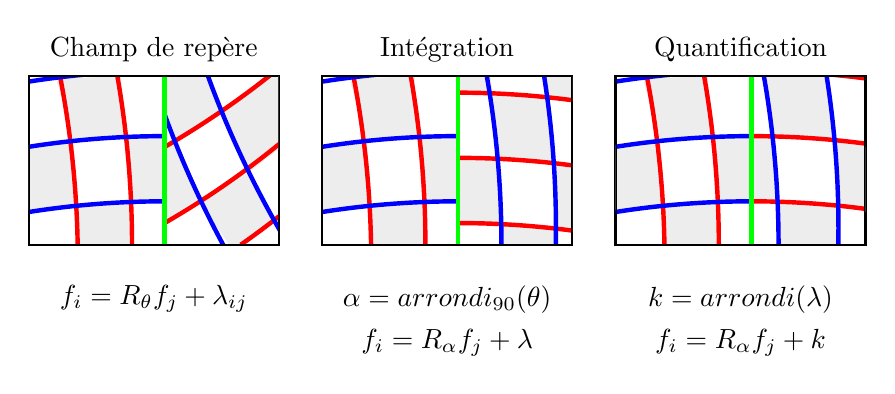
\begin{tikzpicture}[scale=1.38]
		\begin{scope}
			\draw[thick] (-.35, 0) -- (1.95, 0) -- (1.95, 1.55) -- (-.35, 1.55) -- cycle;
			\clip (-.35, 0) -- (1.95, 0) -- (1.95, 1.55) -- (-.35, 1.55) -- cycle;
			\fill[gray!14] (.06, .97) -- (.53, 1) -- (.5, 1.55) -- (-.1, 1.53);
			\fill[gray!14] (.06, .97) -- (-.5, .9) -- (-.5, .3) -- (.1, .37);
			\fill[gray!14] (.1, .37) -- (.57, .4) -- (.58, 0) -- (.1, 0);
			\fill[gray!14] (.57, .4) -- (.9, .4) -- (.9, 1.) -- (.53, 1.);
			\fill[gray!14] (.9, 1.2) -- (.9, 1.55) -- (1.3, 1.55) -- (1.44, 1.24) -- (.98, .96);
			\fill[gray!14] (1.44, 1.24) -- (1.95, 1.6) -- (1.95, .88) -- (1.68, .67);
			\fill[gray!14] (.9, .9) -- (.99, .98) -- (1.2, .42) -- (.9, .22);
			\fill[gray!14] (1.53, -.05) -- (1.2, .42) -- (1.68, .67) -- (1.9, .22);
			\draw[ultra thick, red] (0.1, 0) arc(1:11:9);
			\draw[ultra thick, red] (.6, 0) arc(0:10:9);
			\draw[ultra thick, blue] (.9, 0.4) arc(90:99:8);
			\draw[ultra thick, blue] (.9, 1) arc(90:99:8);
			\draw[ultra thick, blue] (.9, 1.6) arc(90:99:8);
			\draw[ultra thick, red] (.9, .2) arc(-60:-50:8);
			\draw[ultra thick, red] (.9, .9) arc(-60:-51:8);
			\draw[ultra thick, red] (1.6, 0) arc(-55:-51:8);
			\draw[ultra thick, blue] (.9, 1.2) arc(200:209:9);
			\draw[ultra thick, blue] (1.3, 1.55) arc(200:210:9);
			\draw[ultra thick, green] (.9, 0) -- (.9, 1.55);
			\draw[thick] (-.35, 0) -- (1.95, 0) -- (1.95, 1.55) -- (-.35, 1.55) -- cycle;
		\end{scope}
		\node at (.8, 1.8) {Champ de repère};
		\node at (.8, -0.5) {$f_i = R_{\theta} f_j + \lambda_{ij}$};
		\begin{scope}[xshift=2.7cm]
			\draw[thick] (-.35, 0) -- (1.95, 0) -- (1.95, 1.55) -- (-.35, 1.55) -- cycle;
			\clip (-.35, 0) -- (1.95, 0) -- (1.95, 1.55) -- (-.35, 1.55) -- cycle;
			\fill[gray!14] (.06, .97) -- (.53, 1) -- (.5, 1.55) -- (-.1, 1.53);
			\fill[gray!14] (.06, .97) -- (-.5, .9) -- (-.5, .3) -- (.1, .37);
			\fill[gray!14] (.1, .37) -- (.57, .4) -- (.58, 0) -- (.1, 0);
			\fill[gray!14] (.57, .4) -- (.9, .4) -- (.9, 1.) -- (.53, 1.);
			\fill[gray!14] (.9, .2) -- (.9, .8) -- (1.27, .78) -- (1.29, .17);
			\fill[gray!14] (1.8, .16) -- (1.77, .76) -- (1.95, .75) -- (1.95, .12);
			\fill[gray!14] (1.27, .78) -- (1.77, .76) -- (1.74, 1.36) -- (1.22, 1.38);
			\fill[gray!14] (.9, 1.4) -- (1.22, 1.39) -- (1.2, 1.55) -- (.9, 1.55);
			\fill[gray!14] (1.73, 1.34) -- (1.71, 1.55) -- (1.95, 1.55) -- (1.95, 1.32);
			\fill[gray!14] (1.3, 0) -- (1.8, 0) -- (1.8, .14) -- (1.3, .18);
			\draw[ultra thick, red] (0.1, 0) arc(1:11:9);
			\draw[ultra thick, red] (.6, 0) arc(0:10:9);
			\draw[ultra thick, blue] (.9, 0.4) arc(90:99:8);
			\draw[ultra thick, blue] (.9, 1) arc(90:99:8);
			\draw[ultra thick, blue] (.9, 1.6) arc(90:99:8);
			\draw[ultra thick, red] (.9, .2) arc(90:82:8);
			\draw[ultra thick, red] (.9, .8) arc(90:82:8);
			\draw[ultra thick, red] (.9, 1.4) arc(90:82:8);
			\draw[ultra thick, blue] (1.3, 0) arc(0:10:9);
			\draw[ultra thick, blue] (1.8, 0) arc(-1:9:9);
			\draw[ultra thick, green] (.9, 0) -- (.9, 1.55);
			\draw[thick] (-.35, 0) -- (1.95, 0) -- (1.95, 1.55) -- (-.35, 1.55) -- cycle;
		\end{scope}
		\node at (3.5, 1.8) {Intégration};
		\node at (3.5, -0.5) {\green{$\alpha = arrondi_{90}(\theta)$}};
		\node at (3.5, -.9) {$f_i = R_{\green{\alpha}} f_j + \lambda$};
		
		\begin{scope}[xshift=5.4cm]
			\draw[thick] (-.35, 0) -- (1.95, 0) -- (1.95, 1.55) -- (-.35, 1.55) -- cycle;
			\clip (-.35, 0) -- (1.95, 0) -- (1.95, 1.55) -- (-.35, 1.55) -- cycle;
			\fill[gray!14] (.06, .97) -- (.53, 1) -- (.5, 1.55) -- (-.1, 1.53);
			\fill[gray!14] (.06, .97) -- (-.5, .9) -- (-.5, .3) -- (.1, .37);
			\fill[gray!14] (.1, .37) -- (.57, .4) -- (.58, 0) -- (.1, 0);
			\fill[gray!14] (.57, .4) -- (1.13, .4) -- (1.11, 1.) -- (.53, 1.);
			\fill[gray!14] (1.13, .4) -- (1.7, .36) -- (1.7, 0) -- (1.15, 0);
			\fill[gray!14] (1.11, 1.) -- (1.68, .96) -- (1.6, 1.55) -- (1.04, 1.55);
			\fill[gray!14] (1.68, .96) -- (1.95, .9) -- (1.95, .3) -- (1.7, .36);
			\draw[ultra thick, red] (0.1, 0) arc(1:11:9);
			\draw[ultra thick, red] (.6, 0) arc(0:10:9);
			\draw[ultra thick, blue] (.9, 0.4) arc(90:99:8);
			\draw[ultra thick, blue] (.9, 1) arc(90:99:8);
			\draw[ultra thick, blue] (.9, 1.6) arc(90:99:8);
			\draw[ultra thick, red] (.9, .4) arc(90:82:8);
			\draw[ultra thick, red] (.9, 1.) arc(90:82:8);
			\draw[ultra thick, red] (.9, 1.6) arc(90:80:8);
			\draw[ultra thick, blue] (1.15, 0) arc(0:10:9);
			\draw[ultra thick, blue] (1.7, 0) arc(-1:9:9);
			\draw[ultra thick, green] (.9, 0) -- (.9, 1.55);
			\draw[thick] (-.35, 0) -- (1.95, 0) -- (1.95, 1.55) -- (-.35, 1.55) -- cycle;
		\end{scope}
		\node at (6.2, 1.8) {Quantification};
		\node at (6.2, -.5) {\purple{$k = arrondi(\lambda)$}};
		\node at (6.2, -0.9) {$f_i = R_{\green{\alpha}} f_j + \purple{k}$};
	
	\end{tikzpicture}
\end{frame}

\begin{frame}{En 3D: Cubecover pour générer un maillage hexaédrique}
    \begin{center}
		\begin{itemize}
			\item Champ de repère 3D [\cite{huang_boundary_2011}]
			\item Intégration avec Cubecover [\cite{nieser_cubecover_2011}]
			\item Quantification 3D [\cite{bruckler_volume_2022}]
		\end{itemize}
		\vspace{1em}
        \includegraphics[width=\linewidth]{img/cubecover/B34_graphe_interieur.PNG}
		%\begin{itemize}
		%	\item Un graphe de singularité 3D est un ensemble d'arête du maillage tétraédrique en entrée.
		%\end{itemize}
        %\small{
        %    \textit{Cubecover utilise le graphe de singularité d'un champ de repère 3D pour construire un maillage hexaédrique partageant le même graphe de singularité.}
        %}
    \end{center}
\end{frame}
